\section{Entorno de desarrollo software PC}\label{cap:analisis}

En este capítulo se expone la configuración del entorno de programación en Linux, como se estructura el proyecto y las herramientas que el entorno de Linux/Debian ofrece.

La puesta a punto del robot a nivel de software se ha desarrollado en un entorno GNU-Linux utilizando distribuciones Debian-Ubuntu para poder instalar todas las herramientas necesarias para poder desarrollar el software que se va a implantar en el robot. 

\subsection{Sistema operativo Ubuntu}
Con el objetivo de tener todas las herramientas posibles a la hora de desarrollar el proyecto y poder utilizar todas las funcionalidades que un sistema operativo puede ofrecer, se ha desarrollado el proyecto prácticamente en su totalidad utilizando Linux como base del sistema operativo y base de desarrollo tanto en PC como en la CPU que utilizará el robot.

\begin{figure}[h]
    \centering
    
\includegraphics[scale=0.15]{fig/ubuntu.png}
    \caption{Logotipo distribución Ubuntu.}
    \label{fig:mesh1}
\end{figure}

Ubuntu es una de las distribuciones mas famosas del 
\subsection{ROS}
ROS es un framework de código abierto que proporciona una serie de librerías para la gestión de desarrollo software aplicado a robots.

Entre las librerías que ROS ofrece se encuentran librerías orientadas a la abstracción de hardware, gestión de dispositivos de bajo nivel, comunicación entre sistemas... Todas estas funcionalidades que este framework proporciona hacen que la gestión de la arquitectura software del robot sea mucho mas intuitiva y manejable y por lo tanto hacer el proyecto mas escalable y abierto a nuevas funcionalidades.

Otra de la principal ventaja que hace que ROS sea uno de los frameworks mas utilizados para el desarrollo de aplicaciones con robots es la alta capacidad de reutilizar código que ofrece, esto se debe a las diferentes capas de abstracción que se utiliza en el desarrollo que hacen el desarrollo de "nodos" y "paquetes" de ROS sean muy poco o nada dependientes del hardware a utilizar.

\begin{figure}[h]
    \centering
    
\includegraphics[scale=0.2]{fig/ros.jpg}
    \caption{logo ROS framework.}
    \label{fig:mesh1}
\end{figure}

ROS está diseñado para ser lo más ligero posible, esto hace que sea m;as sencillo poder ejecutar este framework con recursos limitados, en este proyecto, ROS estará corriendo sobre una Raspberry Pi, por tanto es otra de las cualidades a tener en cuenta a la hora de escoger herramientas de software aplicadas a este robot.

Hay dos lenguajes soportados para desarrollar paquetes de ROS, se puede desarrollar tanto en C++ como en Python. Esto lo hace aún mas versátil si cabe y más accesible a mas desarrolladores abriendo el campo del desarrollo colaborativo y la reutilización de código.
\subsection{Instalación de paquetes y herramientas necesarias en PC.}
El primer paso para utilizar todas las herramientas de desarrollo necesarias es poner a punto el software que se va a utilizar. Durante todo el proyecto se han desempeñado tareas de programación y elaboración de código, para poder gestionar y llevar un seguimiento del control de versiones del código del proyecto se ha creado un repositorio donde se ha ido subiendo cada un de los diferentes cambios que se van realizando con el paso del tiempo.

La herramienta escogida para realizar el control de versiones ha sido GIT. Una de las ventajas significativas de poder utilizar un software de control de versiones como puede ser GIT, es la portabilidad que le ofrece al código. Al utilizar repositorios como contenedor de todo el código del proyecto, este se puede clonar y ejecutar desde diferentes dispositivo sin ningún problema.

Por tanto, ha resultado ser especialmente útil para poder portar el código entre sistemas operativos así como para poder transportarlo del PC a la Raspberry Pi. De esa forma, todo el proyecto queda contenido en un mismo repositorio, a disposición de todos los usuarios que quieran desarrollar sobre él.

\begin{figure}[h]
    \centering
    
\includegraphics[scale=0.2]{fig/git.png}
    \caption{Logo control de versiones GIT.}
    \label{fig:mesh1}
\end{figure}

Para trabajar con el control de ver siones se debe de seguir una determinada metodología con el objetivo de llevar una desarrollo del proyecto de forma correcta. Generalmente a la hora de desarrollar un proyecto en GIT, se suele hacer de forma colaborativa, donde todo un equipo de desarrollo se verá involucrado en un determinado código. En este caso, solo uno o dos usuarios serán aquellos que hagan modificaciones en el código.

La metodología mas adecuada que se ha escogido para llevar a cabo el proyecto ha sido "Git Flow".
Git Flow es una metodología de trabajo donde el repositorio que aloja el proyecto se estructura en diversas ramas o espacios donde se diferencian diversas partes del código y donde se estructura el código de forma que según la versión o funcionalidad se puede escoger de una forma sencilla. Generalmente la estructura de las diferentes ramas utilizadas es la que se muestra en la FIGURAX.
\begin{figure}[h]
    \centering
    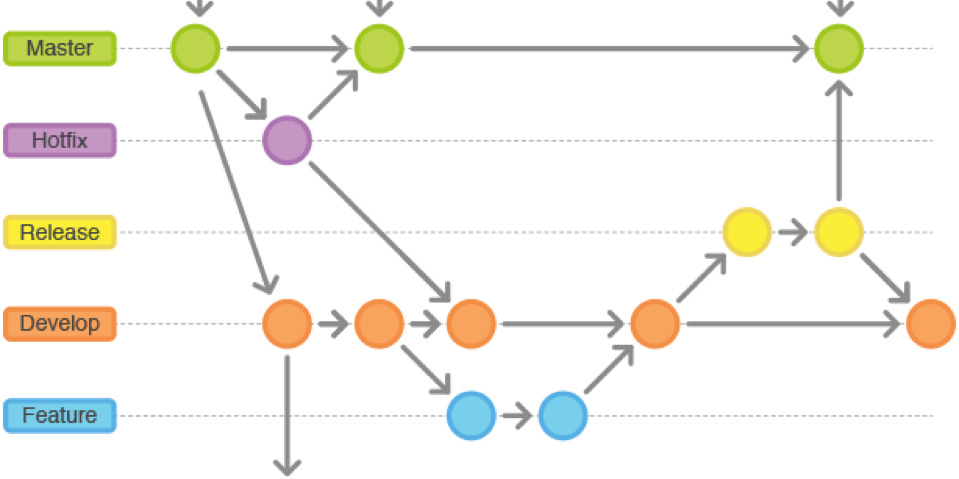
\includegraphics[scale=0.25]{fig/gitFlow.png}
    \caption{Metodología de trabajo ¨Git Flow¨.}
    \label{fig:mesh1}
\end{figure}

Cada una de las ramas alberga el código con las siguientes funcionalidades:
\begin{itemize}
\item Master : Alberga el código que esta actualmente en producción, en este caso alberga el código que se ha utlizado en su versión completamente funcional mas reciente. 
\item Release : Es el último código funcional que se ha enviado para evaluar su calidad y poder enviarlo a producción, también contiene una versión definitiva del código o proyecto a utilizar pero no necesariamente debe de ser el código utilizado en producción.
\item Develop  : Alberga el código que está en actual desarrollo, no necesariamente debe de funcionar a la perfección, aunque es recomendable que todo el código que se pueda descargar de la rama de develop al menos debe de compilar y albergar funcionalidades básicas desarrolladas, aunque en estas se puedan encontrar diferentes bugs. Es la rama donde se encuentra el código antes de mandarlo a la rama de release.
\item Feature : En la rama de feature se desarrollan las nuevas funcionalidades que se van añadir al código.
\end{itemize}


En el caso de este proyecto se ha desglosado en tres ramas, ya que el proyecto no se ha llevado a producción masiva, ha sido suficinete con tener tres ramas diferentes para estructurar de forma correcta el proyecto. En este caso se ha utilizado las ramas "develop" donde se ha ido guardando el código funcional en desarrollo, la rama "feature/" donde se iba desarrollando cada una de las funcionalidades antes de combinarlas con la rama "develop" y por último la rama master, donde se ha ido metiendo el código que era completamente funcional y definitivo.

Otro ámbito importante a la hora de desarrollar el proyecto es poder realizar una correcta depuración de cada una de las partes del proyecto y de cada uno de las diferentes funcionalidades que se van desarrollando a lo largo del proyecto en diferentes ámbitos. Para poder cumplir con este objetivo se han instalado diferentes herramientas que han permitido poder obtener información interesante que verifique el correcto funcionamiento del robot.

En este caso, gran parte de la comunicación establecida entre las diferentes partes del robot, como por ejemplo la comunicación entre el microcontrolador y la Raspberry Pi se han realizado a través de un protocolo UART. La comunicación UART se establece a través de un protocolo serie que se encarga de establecer una comunicación asíncrona donde se envían y reciben datos de forma secuencial a una velocidad determinada, comúnmente llamada "baurate".

\begin{figure}[h]
    \centering
    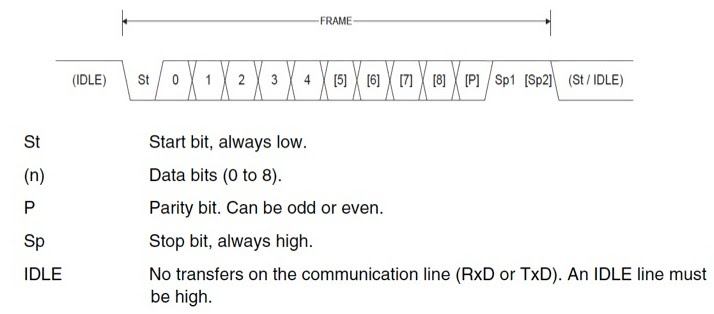
\includegraphics[scale=0.5]{fig/uart.jpg}
    \caption{Resumen protocolo UART.}
    \label{fig:mesh1}
\end{figure}

Para poder llevar a cabo una correcta depuración se ha utilizado un software llamado hercules, el cual permite poder establecer una comunicación entre el ordenador desde el cual se esté trabajando y el dispositivo con el cual se desee comunicar. De este modo, se pueden obtener información para poder conocer en que punto de cada función está en cada momento el código ejecutado y poder mostrar en pantalla la información necesaria para su correcta depuración.

\begin{figure}[h]
    \centering
    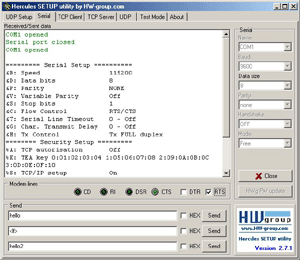
\includegraphics[scale=1.5]{fig/serial1.png}
    \caption{Comucicación serie en Hercules.}
    \label{fig:mesh1}
\end{figure}

El ordenador donde se esté ejecutando el software Hercules debe de poder interpretar la información a través de un USB, por tanto es necesario convertir esa información proveniente de un protocolo UART a un protocolo serie que pueda entender el ordenador.

En este caso se ha utilizado un adaptador capaz de convertir esta información para que pueda establecerse una comunicación en ambos canales y sentidos. El adaptador utilizado se puede encontrar en la siguiente figura.

\begin{figure}[h]
    \centering
    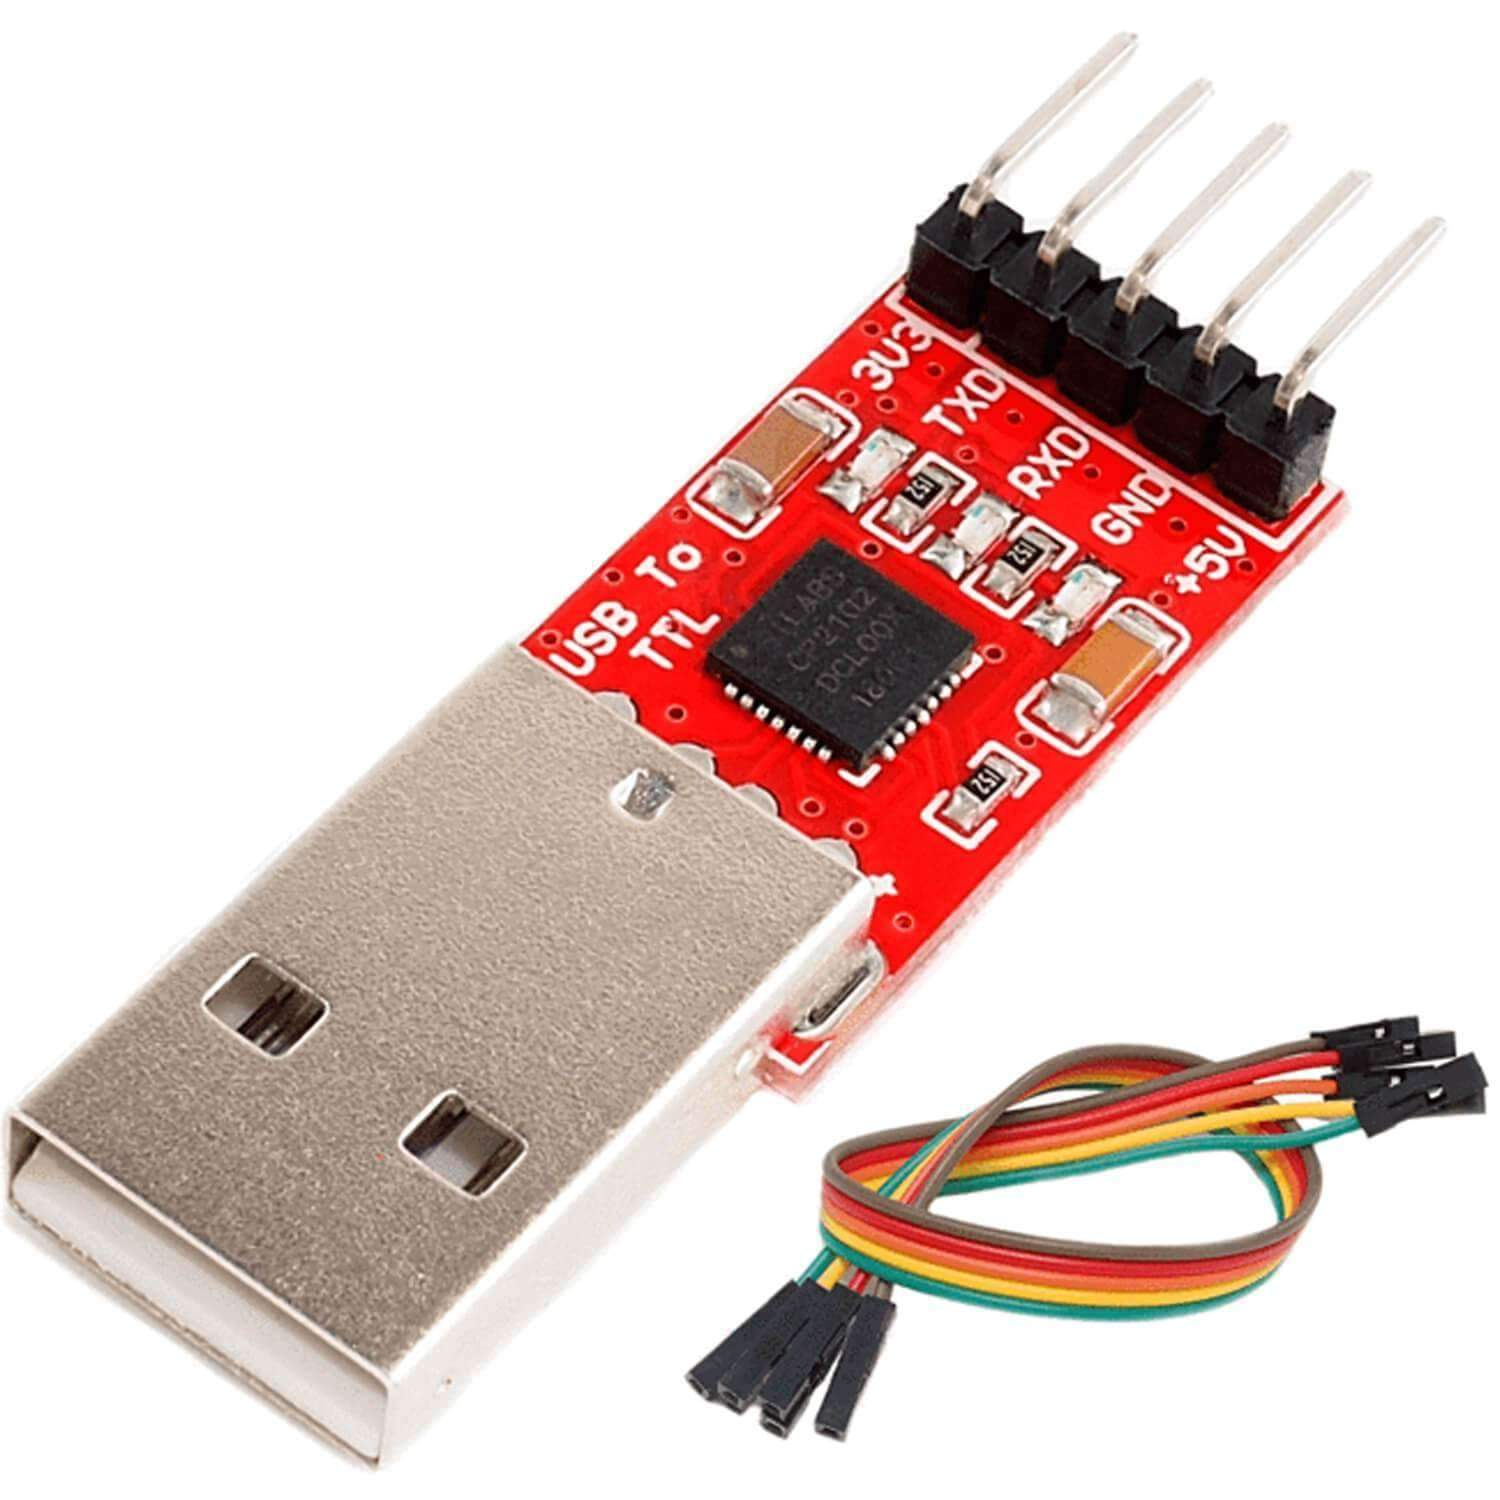
\includegraphics[scale=0.1]{fig/usb_ttl.jpg}
    \caption{Conversor USB-TTL.}
    \label{fig:mesh1}
\end{figure}

Otra herramienta que resulta muy útil a la hora de poder identificar problemas y poder depurar proyectos son los analizadores lógicos. Estos dispositivos permiten poder hacer un análisis a nivel de pines de cada uno de los canales o flujos que se quieran analizar en un proyecto. En ciertas circunstancias, cuando los dispositivos que s están programando no cuentan con herramientas propias de depuración con las que poder monitorizar "logs" o simplemente se quiere cerciorar que el flujo de comunicación funciona de forma correcta. Cualquier canal de comunicación o cualquier pista eléctrica que pueda conducir cualquier tipo de señal puede ser analizada con el analizador lógico, es aquí donde reside la versatilidad de este dispositivo. 

Hay distintos ámbitos en los que un analizador lógico puede ser útil en este proyecto, y en este caso se ha utilizado de diferentes maneras. EL dispositivo utilizado para el proyecto es un analizador lógico genérico que es fácil de encontrar en cualquier tienda de electrónica y con un precio bastante accesible a la mayor parte de los usuarios. El dispositivo se muestra en la figura siguiente.

\begin{figure}[h]
    \centering
    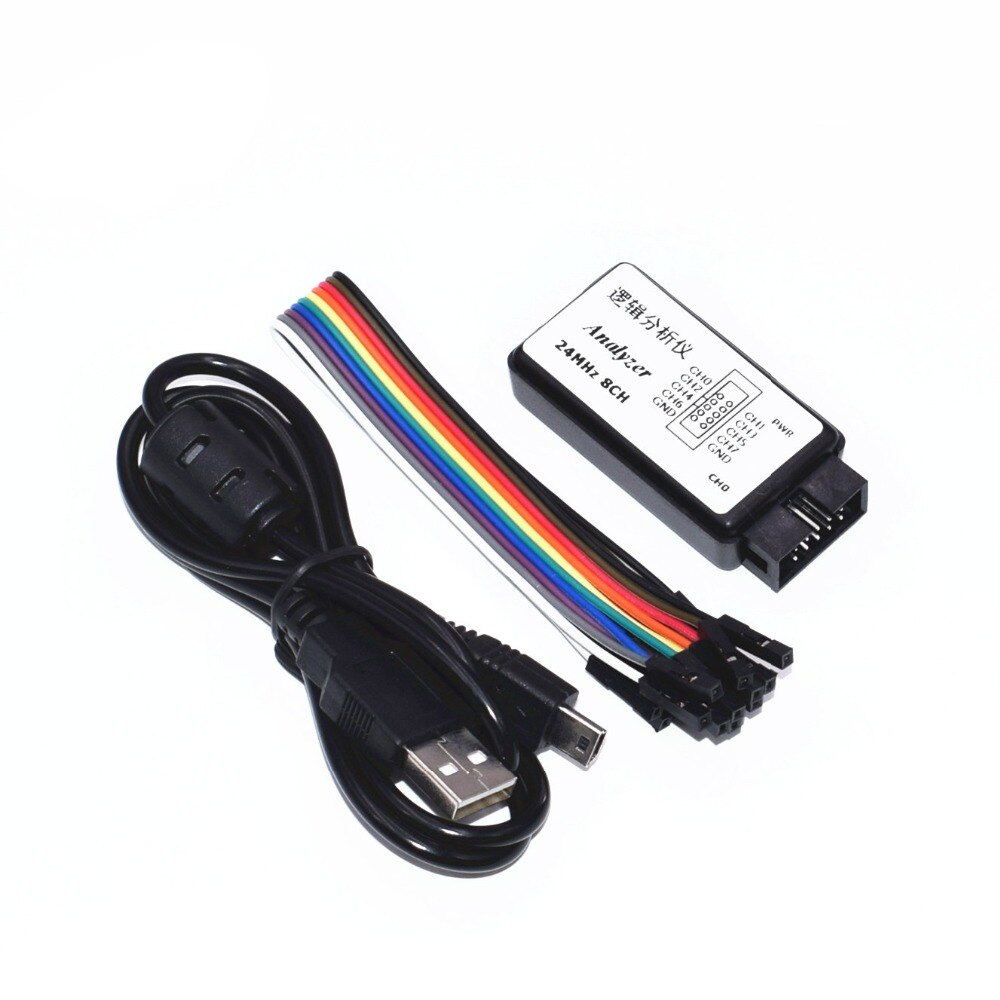
\includegraphics[scale=1]{fig/logic_analyzer.jpg}
    \caption{Analizador lógico utilizado en el proyecto.}
    \label{fig:mesh1}
\end{figure}

Para hacer uso del analizador lógico se necesita un software específico para interpretar la información adquirida por cada uno de los canales del analizador lógico. En este caso se ha utilizado un software libre y abierto llamado sigrok-pulseview, al cual se le deben de instalar los drivers compatibles con el dispositivo que se desea utilizar para poder completar la instalación y poder tener el dispositivo en pleno funcionamiento. Se puede encontrar un ejemplo de funcionamiento en la imagen siguiente.

\begin{figure}[h]
    \centering
    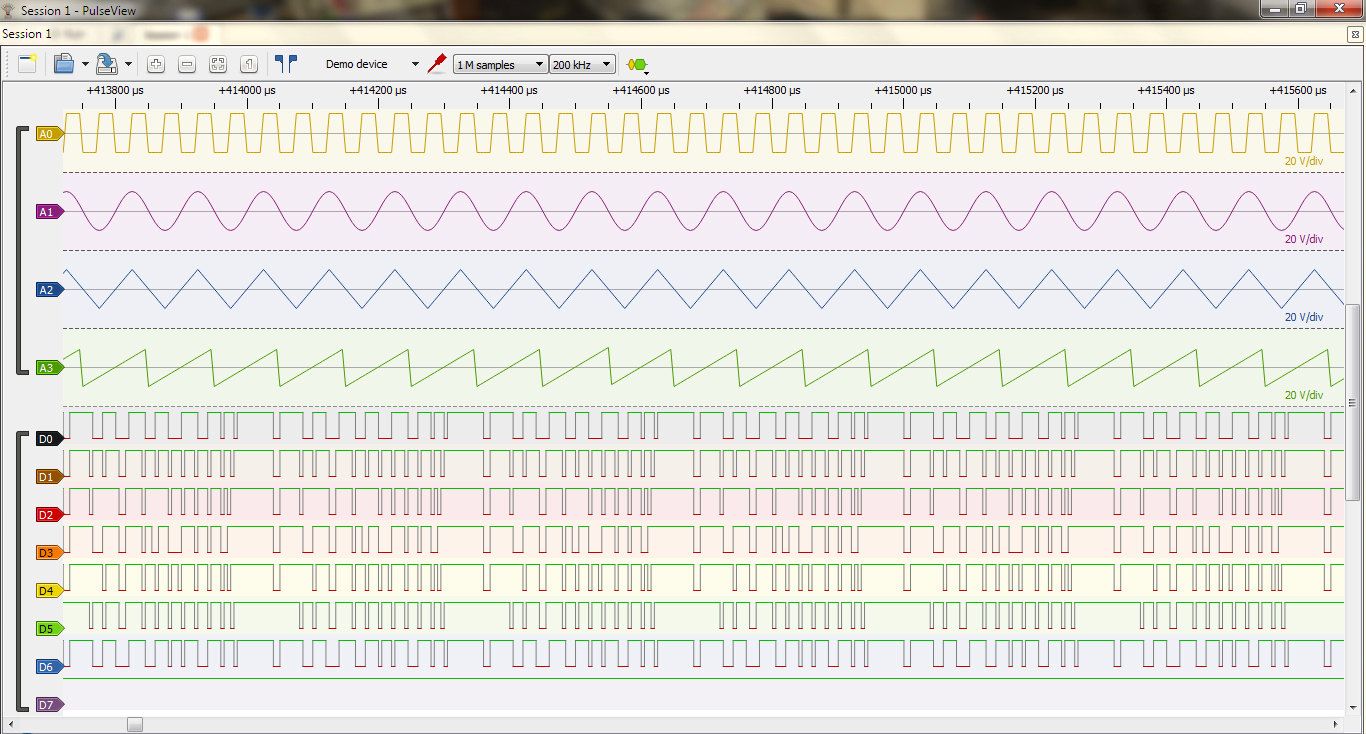
\includegraphics[scale=0.3]{fig/pulseview.jpg}
    \caption{Analizador lógico utilizado en el proyecto.}
    \label{fig:mesh1}
\end{figure}

\subsection{Docker Containers}

Con el propósito de poder replicar el funcionamiento del robot en todos los escenarios posibles de desarrollo, se ha tratado de utilizar un contenedor Docker.
Los contenedores Docker, son utilizados para encapsular y poder replicar y escalar un entorno de desarrollo determinado, donde todos y cada uno de los usuarios que utilicen dicho entorno, puedan tener las mismas herramientas disponibles para dicho desarrollo.

El modelo de robot escogido es el "rosbot description". Este modelo simula un robot de 2 ejes y cuatro ruedas implementado con una sensórica muy similar a la que se va a utilizar en el proyecto.
\subsection{Bash Scripting}

Con el objetivo de comprender como se realiza la detección de objetos, se han de dominar previamente diversos conceptos claves sobre los modelos de inteligencia artificial que se pueden encontrar actualmente en la red y disponen de la capacidad de poder embeberlos en un sistema que sea capaz de procesar esta información en el hardware que lleve el robot utilizado para el proyecto.

El modelo mas utilizado para la detección y segmentación de objetos relacionados con la robótica suelen ser las redes neuronales. Las redes neuronales favorecen el ajuste de una determinada 